\documentclass[]{article}
\usepackage{lmodern}
\usepackage{amssymb,amsmath}
\usepackage{ifxetex,ifluatex}
\usepackage{fixltx2e} % provides \textsubscript
\ifnum 0\ifxetex 1\fi\ifluatex 1\fi=0 % if pdftex
  \usepackage[T1]{fontenc}
  \usepackage[utf8]{inputenc}
\else % if luatex or xelatex
  \ifxetex
    \usepackage{mathspec}
  \else
    \usepackage{fontspec}
  \fi
  \defaultfontfeatures{Ligatures=TeX,Scale=MatchLowercase}
\fi
% use upquote if available, for straight quotes in verbatim environments
\IfFileExists{upquote.sty}{\usepackage{upquote}}{}
% use microtype if available
\IfFileExists{microtype.sty}{%
\usepackage{microtype}
\UseMicrotypeSet[protrusion]{basicmath} % disable protrusion for tt fonts
}{}
\usepackage[margin=1in]{geometry}
\usepackage{hyperref}
\hypersetup{unicode=true,
            pdftitle={project08},
            pdfauthor={Jason Grahn},
            pdfborder={0 0 0},
            breaklinks=true}
\urlstyle{same}  % don't use monospace font for urls
\usepackage{color}
\usepackage{fancyvrb}
\newcommand{\VerbBar}{|}
\newcommand{\VERB}{\Verb[commandchars=\\\{\}]}
\DefineVerbatimEnvironment{Highlighting}{Verbatim}{commandchars=\\\{\}}
% Add ',fontsize=\small' for more characters per line
\usepackage{framed}
\definecolor{shadecolor}{RGB}{248,248,248}
\newenvironment{Shaded}{\begin{snugshade}}{\end{snugshade}}
\newcommand{\KeywordTok}[1]{\textcolor[rgb]{0.13,0.29,0.53}{\textbf{#1}}}
\newcommand{\DataTypeTok}[1]{\textcolor[rgb]{0.13,0.29,0.53}{#1}}
\newcommand{\DecValTok}[1]{\textcolor[rgb]{0.00,0.00,0.81}{#1}}
\newcommand{\BaseNTok}[1]{\textcolor[rgb]{0.00,0.00,0.81}{#1}}
\newcommand{\FloatTok}[1]{\textcolor[rgb]{0.00,0.00,0.81}{#1}}
\newcommand{\ConstantTok}[1]{\textcolor[rgb]{0.00,0.00,0.00}{#1}}
\newcommand{\CharTok}[1]{\textcolor[rgb]{0.31,0.60,0.02}{#1}}
\newcommand{\SpecialCharTok}[1]{\textcolor[rgb]{0.00,0.00,0.00}{#1}}
\newcommand{\StringTok}[1]{\textcolor[rgb]{0.31,0.60,0.02}{#1}}
\newcommand{\VerbatimStringTok}[1]{\textcolor[rgb]{0.31,0.60,0.02}{#1}}
\newcommand{\SpecialStringTok}[1]{\textcolor[rgb]{0.31,0.60,0.02}{#1}}
\newcommand{\ImportTok}[1]{#1}
\newcommand{\CommentTok}[1]{\textcolor[rgb]{0.56,0.35,0.01}{\textit{#1}}}
\newcommand{\DocumentationTok}[1]{\textcolor[rgb]{0.56,0.35,0.01}{\textbf{\textit{#1}}}}
\newcommand{\AnnotationTok}[1]{\textcolor[rgb]{0.56,0.35,0.01}{\textbf{\textit{#1}}}}
\newcommand{\CommentVarTok}[1]{\textcolor[rgb]{0.56,0.35,0.01}{\textbf{\textit{#1}}}}
\newcommand{\OtherTok}[1]{\textcolor[rgb]{0.56,0.35,0.01}{#1}}
\newcommand{\FunctionTok}[1]{\textcolor[rgb]{0.00,0.00,0.00}{#1}}
\newcommand{\VariableTok}[1]{\textcolor[rgb]{0.00,0.00,0.00}{#1}}
\newcommand{\ControlFlowTok}[1]{\textcolor[rgb]{0.13,0.29,0.53}{\textbf{#1}}}
\newcommand{\OperatorTok}[1]{\textcolor[rgb]{0.81,0.36,0.00}{\textbf{#1}}}
\newcommand{\BuiltInTok}[1]{#1}
\newcommand{\ExtensionTok}[1]{#1}
\newcommand{\PreprocessorTok}[1]{\textcolor[rgb]{0.56,0.35,0.01}{\textit{#1}}}
\newcommand{\AttributeTok}[1]{\textcolor[rgb]{0.77,0.63,0.00}{#1}}
\newcommand{\RegionMarkerTok}[1]{#1}
\newcommand{\InformationTok}[1]{\textcolor[rgb]{0.56,0.35,0.01}{\textbf{\textit{#1}}}}
\newcommand{\WarningTok}[1]{\textcolor[rgb]{0.56,0.35,0.01}{\textbf{\textit{#1}}}}
\newcommand{\AlertTok}[1]{\textcolor[rgb]{0.94,0.16,0.16}{#1}}
\newcommand{\ErrorTok}[1]{\textcolor[rgb]{0.64,0.00,0.00}{\textbf{#1}}}
\newcommand{\NormalTok}[1]{#1}
\usepackage{graphicx,grffile}
\makeatletter
\def\maxwidth{\ifdim\Gin@nat@width>\linewidth\linewidth\else\Gin@nat@width\fi}
\def\maxheight{\ifdim\Gin@nat@height>\textheight\textheight\else\Gin@nat@height\fi}
\makeatother
% Scale images if necessary, so that they will not overflow the page
% margins by default, and it is still possible to overwrite the defaults
% using explicit options in \includegraphics[width, height, ...]{}
\setkeys{Gin}{width=\maxwidth,height=\maxheight,keepaspectratio}
\IfFileExists{parskip.sty}{%
\usepackage{parskip}
}{% else
\setlength{\parindent}{0pt}
\setlength{\parskip}{6pt plus 2pt minus 1pt}
}
\setlength{\emergencystretch}{3em}  % prevent overfull lines
\providecommand{\tightlist}{%
  \setlength{\itemsep}{0pt}\setlength{\parskip}{0pt}}
\setcounter{secnumdepth}{0}
% Redefines (sub)paragraphs to behave more like sections
\ifx\paragraph\undefined\else
\let\oldparagraph\paragraph
\renewcommand{\paragraph}[1]{\oldparagraph{#1}\mbox{}}
\fi
\ifx\subparagraph\undefined\else
\let\oldsubparagraph\subparagraph
\renewcommand{\subparagraph}[1]{\oldsubparagraph{#1}\mbox{}}
\fi

%%% Use protect on footnotes to avoid problems with footnotes in titles
\let\rmarkdownfootnote\footnote%
\def\footnote{\protect\rmarkdownfootnote}

%%% Change title format to be more compact
\usepackage{titling}

% Create subtitle command for use in maketitle
\newcommand{\subtitle}[1]{
  \posttitle{
    \begin{center}\large#1\end{center}
    }
}

\setlength{\droptitle}{-2em}

  \title{project08}
    \pretitle{\vspace{\droptitle}\centering\huge}
  \posttitle{\par}
    \author{Jason Grahn}
    \preauthor{\centering\large\emph}
  \postauthor{\par}
      \predate{\centering\large\emph}
  \postdate{\par}
    \date{2/24/2019}


\begin{document}
\maketitle

\begin{Shaded}
\begin{Highlighting}[]
\KeywordTok{library}\NormalTok{(readr)}
\NormalTok{mydata <-}\StringTok{ }\KeywordTok{read_csv}\NormalTok{(here}\OperatorTok{::}\KeywordTok{here}\NormalTok{(}\StringTok{"project08/binary.csv"}\NormalTok{))}
\end{Highlighting}
\end{Shaded}

\begin{verbatim}
## Parsed with column specification:
## cols(
##   admit = col_double(),
##   gre = col_double(),
##   gpa = col_double(),
##   rank = col_double()
## )
\end{verbatim}

\begin{Shaded}
\begin{Highlighting}[]
\KeywordTok{summary}\NormalTok{(mydata) }
\end{Highlighting}
\end{Shaded}

\begin{verbatim}
##      admit             gre             gpa             rank      
##  Min.   :0.0000   Min.   :220.0   Min.   :2.260   Min.   :1.000  
##  1st Qu.:0.0000   1st Qu.:520.0   1st Qu.:3.130   1st Qu.:2.000  
##  Median :0.0000   Median :580.0   Median :3.395   Median :2.000  
##  Mean   :0.3175   Mean   :587.7   Mean   :3.390   Mean   :2.485  
##  3rd Qu.:1.0000   3rd Qu.:660.0   3rd Qu.:3.670   3rd Qu.:3.000  
##  Max.   :1.0000   Max.   :800.0   Max.   :4.000   Max.   :4.000
\end{verbatim}

\begin{Shaded}
\begin{Highlighting}[]
\NormalTok{## Summary shows gre and gpa appear to be approximately normally distributed.}

\KeywordTok{sapply}\NormalTok{(mydata, sd) }
\end{Highlighting}
\end{Shaded}

\begin{verbatim}
##       admit         gre         gpa        rank 
##   0.4660867 115.5165364   0.3805668   0.9444602
\end{verbatim}

\begin{Shaded}
\begin{Highlighting}[]
\KeywordTok{xtabs}\NormalTok{(}\OperatorTok{~}\StringTok{ }\NormalTok{admit }\OperatorTok{+}\StringTok{ }\NormalTok{rank, }\DataTypeTok{data =}\NormalTok{ mydata)}
\end{Highlighting}
\end{Shaded}

\begin{verbatim}
##      rank
## admit  1  2  3  4
##     0 28 97 93 55
##     1 33 54 28 12
\end{verbatim}

Here we've built a crosstab for each college rank and the count of those
that are admitted to it. There are no \textbf{0} cells, so we can
proceed.

\begin{Shaded}
\begin{Highlighting}[]
\NormalTok{mydata}\OperatorTok{$}\NormalTok{rank <-}\StringTok{ }\KeywordTok{factor}\NormalTok{(mydata}\OperatorTok{$}\NormalTok{rank) }
\NormalTok{mylogit <-}\StringTok{ }\KeywordTok{glm}\NormalTok{(admit }\OperatorTok{~}\StringTok{ }\NormalTok{gre }\OperatorTok{+}\StringTok{ }\NormalTok{gpa }\OperatorTok{+}\StringTok{ }\NormalTok{rank, }\DataTypeTok{data =}\NormalTok{ mydata, }\DataTypeTok{family =} \StringTok{"binomial"}\NormalTok{)}
\KeywordTok{summary}\NormalTok{(mylogit)}
\end{Highlighting}
\end{Shaded}

\begin{verbatim}
## 
## Call:
## glm(formula = admit ~ gre + gpa + rank, family = "binomial", 
##     data = mydata)
## 
## Deviance Residuals: 
##     Min       1Q   Median       3Q      Max  
## -1.6268  -0.8662  -0.6388   1.1490   2.0790  
## 
## Coefficients:
##              Estimate Std. Error z value Pr(>|z|)    
## (Intercept) -3.989979   1.139951  -3.500 0.000465 ***
## gre          0.002264   0.001094   2.070 0.038465 *  
## gpa          0.804038   0.331819   2.423 0.015388 *  
## rank2       -0.675443   0.316490  -2.134 0.032829 *  
## rank3       -1.340204   0.345306  -3.881 0.000104 ***
## rank4       -1.551464   0.417832  -3.713 0.000205 ***
## ---
## Signif. codes:  0 '***' 0.001 '**' 0.01 '*' 0.05 '.' 0.1 ' ' 1
## 
## (Dispersion parameter for binomial family taken to be 1)
## 
##     Null deviance: 499.98  on 399  degrees of freedom
## Residual deviance: 458.52  on 394  degrees of freedom
## AIC: 470.52
## 
## Number of Fisher Scoring iterations: 4
\end{verbatim}

This is the output for the generalized linear model (GLM). We're given
the forumula for the model and an evaluation of the model. Rank3 and
rank4 are both highly significant at practically 0 alpha; while rank2,
gpa, and gre are only significant at .05 alpha.

\begin{Shaded}
\begin{Highlighting}[]
\NormalTok{## CIs using profiled log-likelihood }
\KeywordTok{round}\NormalTok{(}\KeywordTok{confint}\NormalTok{(mylogit), }\DecValTok{4}\NormalTok{)}
\end{Highlighting}
\end{Shaded}

\begin{verbatim}
## Waiting for profiling to be done...
\end{verbatim}

\begin{verbatim}
##               2.5 %  97.5 %
## (Intercept) -6.2716 -1.7925
## gre          0.0001  0.0044
## gpa          0.1603  1.4641
## rank2       -1.3009 -0.0567
## rank3       -2.0277 -0.6704
## rank4       -2.4000 -0.7535
\end{verbatim}

\begin{Shaded}
\begin{Highlighting}[]
\NormalTok{## CIs using standard errors }
\KeywordTok{round}\NormalTok{(}\KeywordTok{confint.default}\NormalTok{(mylogit),}\DecValTok{4}\NormalTok{)}
\end{Highlighting}
\end{Shaded}

\begin{verbatim}
##               2.5 %  97.5 %
## (Intercept) -6.2242 -1.7557
## gre          0.0001  0.0044
## gpa          0.1537  1.4544
## rank2       -1.2958 -0.0551
## rank3       -2.0170 -0.6634
## rank4       -2.3704 -0.7325
\end{verbatim}

Here we have confidence intervals for each of the linear
coefficientsthat are provided in the GLM above. With a logistic model we
\emph{should} be utilizing the profiled log-likelihood function.

\begin{Shaded}
\begin{Highlighting}[]
\KeywordTok{wald.test}\NormalTok{(}\DataTypeTok{b =} \KeywordTok{coef}\NormalTok{(mylogit), }\DataTypeTok{Sigma =} \KeywordTok{vcov}\NormalTok{(mylogit), }\DataTypeTok{Terms =} \DecValTok{4}\OperatorTok{:}\DecValTok{6}\NormalTok{)}
\end{Highlighting}
\end{Shaded}

\begin{verbatim}
## Wald test:
## ----------
## 
## Chi-squared test:
## X2 = 20.9, df = 3, P(> X2) = 0.00011
\end{verbatim}

The wald test shows the effect of rank overall. Our chi-squared test
statistic is 20.9,and the three degrees of freedom is associated to a
p-value of nearly zero (0.00011). This indicates that that the effect of
rank is statistically significant.

\begin{Shaded}
\begin{Highlighting}[]
\NormalTok{l <-}\StringTok{ }\KeywordTok{cbind}\NormalTok{(}\DecValTok{0}\NormalTok{,}\DecValTok{0}\NormalTok{,}\DecValTok{0}\NormalTok{,}\DecValTok{1}\NormalTok{,}\OperatorTok{-}\DecValTok{1}\NormalTok{,}\DecValTok{0}\NormalTok{) }
\KeywordTok{wald.test}\NormalTok{(}\DataTypeTok{b =} \KeywordTok{coef}\NormalTok{(mylogit), }\DataTypeTok{Sigma =} \KeywordTok{vcov}\NormalTok{(mylogit), }\DataTypeTok{L =}\NormalTok{ l)}
\end{Highlighting}
\end{Shaded}

\begin{verbatim}
## Wald test:
## ----------
## 
## Chi-squared test:
## X2 = 5.5, df = 1, P(> X2) = 0.019
\end{verbatim}

Using ``l'' we've done a different wald test here, that results with a
chi-square statistic at 5.5. This has an associated p-value of 0.019.
This tells us that difference between rank2 and rank3 is also
statistically significant.

\begin{Shaded}
\begin{Highlighting}[]
\NormalTok{## odds ratios only }
\KeywordTok{round}\NormalTok{(}\KeywordTok{exp}\NormalTok{(}\KeywordTok{coef}\NormalTok{(mylogit)), }\DecValTok{4}\NormalTok{)}
\end{Highlighting}
\end{Shaded}

\begin{verbatim}
## (Intercept)         gre         gpa       rank2       rank3       rank4 
##      0.0185      1.0023      2.2345      0.5089      0.2618      0.2119
\end{verbatim}

\begin{Shaded}
\begin{Highlighting}[]
\NormalTok{## odds ratios and 95% CI }
\KeywordTok{round}\NormalTok{(}\KeywordTok{exp}\NormalTok{(}\KeywordTok{cbind}\NormalTok{(}\DataTypeTok{OR =} \KeywordTok{coef}\NormalTok{(mylogit), }\KeywordTok{confint}\NormalTok{(mylogit))), }\DecValTok{4}\NormalTok{)}
\end{Highlighting}
\end{Shaded}

\begin{verbatim}
## Waiting for profiling to be done...
\end{verbatim}

\begin{verbatim}
##                 OR  2.5 % 97.5 %
## (Intercept) 0.0185 0.0019 0.1665
## gre         1.0023 1.0001 1.0044
## gpa         2.2345 1.1739 4.3238
## rank2       0.5089 0.2723 0.9448
## rank3       0.2618 0.1316 0.5115
## rank4       0.2119 0.0907 0.4707
\end{verbatim}

In this block of code we're exponentiating the coefficients in order to
interpret them as odds-ratios. This allows us to say that increasing GPA
by one unit increases the \emph{odds} of being admitted into one of
these schools increases by a 2.23. This is against being not admitted at
all.

\begin{Shaded}
\begin{Highlighting}[]
\NormalTok{newdata1 <-}\StringTok{ }\KeywordTok{with}\NormalTok{(mydata, }
                 \KeywordTok{data.frame}\NormalTok{(}\DataTypeTok{gre =} \KeywordTok{mean}\NormalTok{(gre), }
                            \DataTypeTok{gpa =} \KeywordTok{mean}\NormalTok{(gpa), }
                            \DataTypeTok{rank =} \KeywordTok{factor}\NormalTok{(}\DecValTok{1}\OperatorTok{:}\DecValTok{4}\NormalTok{))) }
\NormalTok{## view data frame }
\NormalTok{newdata1}
\end{Highlighting}
\end{Shaded}

\begin{verbatim}
##     gre    gpa rank
## 1 587.7 3.3899    1
## 2 587.7 3.3899    2
## 3 587.7 3.3899    3
## 4 587.7 3.3899    4
\end{verbatim}

\begin{Shaded}
\begin{Highlighting}[]
\NormalTok{newdata1}\OperatorTok{$}\NormalTok{rankP <-}\StringTok{ }\KeywordTok{predict}\NormalTok{(mylogit, }\DataTypeTok{newdata =}\NormalTok{ newdata1, }\DataTypeTok{type =} \StringTok{"response"}\NormalTok{) }
\NormalTok{newdata1}
\end{Highlighting}
\end{Shaded}

\begin{verbatim}
##     gre    gpa rank     rankP
## 1 587.7 3.3899    1 0.5166016
## 2 587.7 3.3899    2 0.3522846
## 3 587.7 3.3899    3 0.2186120
## 4 587.7 3.3899    4 0.1846684
\end{verbatim}

To interpret the values in the new dataframe, we have to remember these
are probability factors. The probability for being accepted into a
school given the mean \texttt{gre} and mean \texttt{gpa} and coming from
a rank1 school is 0.5166016. For students of so-called ``lower tier''
rank4 schools, the probability is 0.1846684 controlling for the same
mean \texttt{gre} and \texttt{gpa}. One way this can be interpreted is
that college is a sociological ``classist'' issue and should be made
free for all based on merit, not the \emph{school} that someone comes
from.

\begin{Shaded}
\begin{Highlighting}[]
\NormalTok{newdata2 <-}\StringTok{ }\KeywordTok{with}\NormalTok{(mydata, }
                 \KeywordTok{data.frame}\NormalTok{(}\DataTypeTok{gre =} \KeywordTok{rep}\NormalTok{(}\KeywordTok{seq}\NormalTok{(}\DataTypeTok{from =} \DecValTok{200}\NormalTok{, }\DataTypeTok{to =} \DecValTok{800}\NormalTok{, }\DataTypeTok{length.out =} \DecValTok{100}\NormalTok{), }\DecValTok{4}\NormalTok{), }
                            \DataTypeTok{gpa =} \KeywordTok{mean}\NormalTok{(gpa), }
                            \DataTypeTok{rank =} \KeywordTok{factor}\NormalTok{(}\KeywordTok{rep}\NormalTok{(}\DecValTok{1}\OperatorTok{:}\DecValTok{4}\NormalTok{, }\DataTypeTok{each =} \DecValTok{100}\NormalTok{))))}
\end{Highlighting}
\end{Shaded}

\begin{Shaded}
\begin{Highlighting}[]
\NormalTok{newdata3 <-}\StringTok{ }\KeywordTok{cbind}\NormalTok{(newdata2, }
                  \KeywordTok{predict}\NormalTok{(mylogit, }
                          \DataTypeTok{newdata =}\NormalTok{ newdata2, }
                          \DataTypeTok{type=}\StringTok{"link"}\NormalTok{, }
                          \DataTypeTok{se=}\OtherTok{TRUE}\NormalTok{)) }

\NormalTok{newdata3 <-}\StringTok{ }\KeywordTok{within}\NormalTok{(newdata3, \{ }
\NormalTok{  PredictedProb <-}\StringTok{ }\KeywordTok{plogis}\NormalTok{(fit) }
\NormalTok{  LL <-}\StringTok{ }\KeywordTok{plogis}\NormalTok{(fit }\OperatorTok{-}\StringTok{ }\NormalTok{(}\FloatTok{1.96} \OperatorTok{*}\StringTok{ }\NormalTok{se.fit)) }
\NormalTok{  UL <-}\StringTok{ }\KeywordTok{plogis}\NormalTok{(fit }\OperatorTok{+}\StringTok{ }\NormalTok{(}\FloatTok{1.96} \OperatorTok{*}\StringTok{ }\NormalTok{se.fit)) \}) }

\NormalTok{## view first few rows of final dataset }
\KeywordTok{head}\NormalTok{(newdata3)}
\end{Highlighting}
\end{Shaded}

\begin{verbatim}
##        gre    gpa rank        fit    se.fit residual.scale        UL
## 1 200.0000 3.3899    1 -0.8114870 0.5147714              1 0.5492064
## 2 206.0606 3.3899    1 -0.7977632 0.5090986              1 0.5498513
## 3 212.1212 3.3899    1 -0.7840394 0.5034491              1 0.5505074
## 4 218.1818 3.3899    1 -0.7703156 0.4978239              1 0.5511750
## 5 224.2424 3.3899    1 -0.7565919 0.4922237              1 0.5518545
## 6 230.3030 3.3899    1 -0.7428681 0.4866494              1 0.5525464
##          LL PredictedProb
## 1 0.1393812     0.3075737
## 2 0.1423880     0.3105042
## 3 0.1454429     0.3134499
## 4 0.1485460     0.3164108
## 5 0.1516973     0.3193867
## 6 0.1548966     0.3223773
\end{verbatim}

All we're making here is an expanded data frame, applying the admission
prediction probabilities to the dataset.

\begin{Shaded}
\begin{Highlighting}[]
\KeywordTok{ggplot}\NormalTok{(newdata3, }\KeywordTok{aes}\NormalTok{(}\DataTypeTok{x =}\NormalTok{ gre, }\DataTypeTok{y =}\NormalTok{ PredictedProb)) }\OperatorTok{+}\StringTok{ }
\StringTok{  }\KeywordTok{geom_ribbon}\NormalTok{(}\KeywordTok{aes}\NormalTok{(}\DataTypeTok{ymin =}\NormalTok{ LL, }\DataTypeTok{ymax =}\NormalTok{ UL, }\DataTypeTok{fill =}\NormalTok{ rank), }\DataTypeTok{alpha =}\NormalTok{ .}\DecValTok{2}\NormalTok{) }\OperatorTok{+}\StringTok{ }
\StringTok{  }\KeywordTok{geom_line}\NormalTok{(}\KeywordTok{aes}\NormalTok{(}\DataTypeTok{colour =}\NormalTok{ rank), }\DataTypeTok{size=}\FloatTok{1.5}\NormalTok{)}
\end{Highlighting}
\end{Shaded}

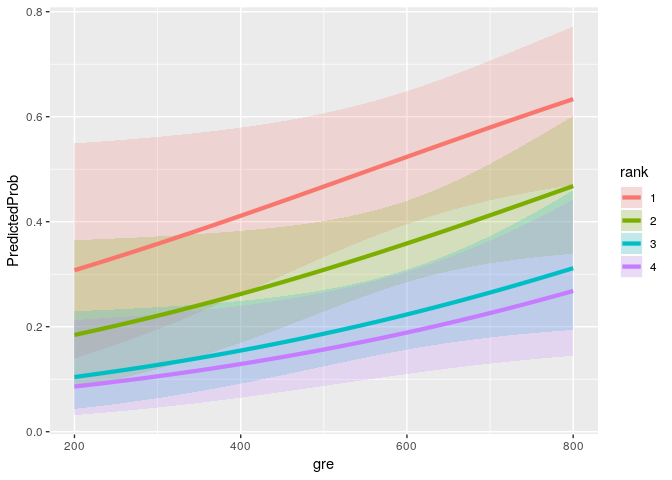
\includegraphics{project8_files/figure-latex/unnamed-chunk-12-1.pdf}

Now we get into some visual fun. With this plot we see the predicted
probability for admission increases with \texttt{gre} score is true for
each rank school. However, rank1 schools have a much higher probability.
Confidence intervals generally overlap, which shows us that it's
possible for a rank4 school attendee to reach SOME of the admission
probability of a rank1 attendee, but only barely, and only at the low
end. The Merits of GRE-based admission are nearly copletely lost at the
high-end of scores. College admission is a class issue.

\begin{Shaded}
\begin{Highlighting}[]
\KeywordTok{with}\NormalTok{(mylogit, null.deviance }\OperatorTok{-}\StringTok{ }\NormalTok{deviance)}
\end{Highlighting}
\end{Shaded}

\begin{verbatim}
## [1] 41.45903
\end{verbatim}

\begin{Shaded}
\begin{Highlighting}[]
\KeywordTok{with}\NormalTok{(mylogit, df.null }\OperatorTok{-}\StringTok{ }\NormalTok{df.residual)}
\end{Highlighting}
\end{Shaded}

\begin{verbatim}
## [1] 5
\end{verbatim}

\begin{Shaded}
\begin{Highlighting}[]
\KeywordTok{with}\NormalTok{(mylogit, }\KeywordTok{pchisq}\NormalTok{(null.deviance }\OperatorTok{-}\StringTok{ }\NormalTok{deviance, df.null }\OperatorTok{-}\StringTok{ }\NormalTok{df.residual, }\DataTypeTok{lower.tail =} \OtherTok{FALSE}\NormalTok{))}
\end{Highlighting}
\end{Shaded}

\begin{verbatim}
## [1] 7.578194e-08
\end{verbatim}

The chi-square is 41.4590251 and has 5 degrees of freedom. This provides
a p-value of 7.5781942\times 10\^{}\{-8\}. This is obviously much less
than any measurable test for fit. The interpretation is that the model
fits better than any random selection.

\begin{Shaded}
\begin{Highlighting}[]
\KeywordTok{logLik}\NormalTok{(mylogit)}
\end{Highlighting}
\end{Shaded}

\begin{verbatim}
## 'log Lik.' -229.2587 (df=6)
\end{verbatim}


\end{document}
